% !TEX TS-program = pdflatex
% !TEX encoding = UTF-8 Unicode

% This is a simple template for a LaTeX document using the "article" class.
% See "book", "report", "letter" for other types of document.

\documentclass[12pt]{article} % use larger type; default would be 10pt

\usepackage[utf8]{inputenc} % set input encoding (not needed with XeLaTeX)
\usepackage{amssymb}
%%% Examples of Article customizations
% These packages are optional, depending whether you want the features they provide.
% See the LaTeX Companion or other references for full information.

%%% PAGE DIMENSIONS
\usepackage{geometry} % to change the page dimensions
\usepackage{setspace}
\geometry{a4paper} % or letterpaper (US) or a5paper or....
\geometry{margin=1in} % for example, change the margins to 2 inches all round
% \geometry{landscape} % set up the page for landscape
%   read geometry.pdf for detailed page layout information

\usepackage{graphicx} % support the \includegraphics command and options

% \usepackage[parfill]{parskip} % Activate to begin paragraphs with an empty line rather than an indent

%%% PACKAGES
\usepackage{booktabs} % for much better looking tables
\usepackage{array} % for better arrays (eg matrices) in maths
\usepackage{paralist} % very flexible & customisable lists (eg. enumerate/itemize, etc.)
\usepackage{verbatim} % adds environment for commenting out blocks of text & for better verbatim
\usepackage{subfig} % make it possible to include more than one captioned figure/table in a single float
% These packages are all incorporated in the memoir class to one degree or another...

%%% HEADERS & FOOTERS
\usepackage{fancyhdr} % This should be set AFTER setting up the page geometry
\pagestyle{fancy} % options: empty , plain , fancy
\renewcommand{\headrulewidth}{0pt} % customise the layout...
\lhead{}\chead{}\rhead{}
\lfoot{}\cfoot{\thepage}\rfoot{}

%%% SECTION TITLE APPEARANCE
\usepackage{sectsty}
\allsectionsfont{\sffamily\mdseries\upshape} % (See the fntguide.pdf for font help)
% (This matches ConTeXt defaults)

%%% ToC (table of contents) APPEARANCE
\usepackage[nottoc,notlof,notlot]{tocbibind} % Put the bibliography in the ToC
\usepackage[titles,subfigure]{tocloft} % Alter the style of the Table of Contents
\renewcommand{\cftsecfont}{\rmfamily\mdseries\upshape}
\renewcommand{\cftsecpagefont}{\rmfamily\mdseries\upshape} % No bold!

%%% END Article customizations

%%% The "real" document content comes below...

\title{1.2 Hess's Law}
\author{Peter Zhang}
%\date{} % Activate to display a given date or no date (if empty),
         % otherwise the current date is printed 

\doublespacing
\begin{document}
\maketitle

\pagebreak

\tableofcontents

\pagebreak

% start document
\section{Hess's Law}

\subsection{Issues with Certain Reactions}
In certain reactions, it is not possible to measure the change in temperature, for instance: `find temp change during combustion of Mg over fire`


Therefore, Hess's Law lets us calculate for it.

\subsection{How to use}

Given a series of formulas, one can solve the system of equations to find the enthalpy of a desired reaction. For instance, given the following equations:

\begin{enumerate}
\item \textbf{Desired:} $Mg + \frac{1}{2}O_2 \rightarrow MgO$ -$\triangle{H} = ?$
\item $Mg + 2HCl_{(g)} \rightarrow MgCl_2$ -$\triangle{H} = -231.2kJ/mol$
\item $MgCl_2 + H_2O \rightarrow MgO + 2HCl$ -$\triangle{H} = +95kJ/mol$
\item $H_2 + \frac{1}{2}O_2 \rightarrow 2H_2O$ -$\triangle{H} = -571.6kJ/mol$
\end{enumerate}

\subsection{Manipulating Reaction Equations}

\begin{enumerate}
\item Reversing
\item Multiplying
\item Dividing
\end{enumerate}

\singlespace

\subsubsection{Reversing Equations}

When reversing equations, multiply everything by -1. This means that everything will be flipped: the products and reactants are flipped and the enthalpy is multiplied by -1.

$$[1]\ 2F_2 + O_2 = 2OF_2 \  |\ \triangle{H} = 98.8kJ/mol$$

not negative anymore bc we swapped/reversed equation

\subsubsection{Multiplying Equations}

When multiplying equations, multiply everything by a constant. Only constants, such as 1, 2, 3, etc. Negative numbers also work: that is how Reversing equations work. Make sure to multiply enthalpy as well!

$$[2]\ ClF+O_2 = Cl_2O + OF_2\ |\ \triangle{H} = 205.6kJ/mol$$

x2

$$[2]\ 2ClF + O_2 = Cl_2O + OF_2 \ |\ \triangle{H} = 416.2kJ/mol$$

\subsubsection{Dividing Equations}

When dividing equations, just divide everything by a constnat. Make sure to divide enthalpy as well!

$$[3]\ ClF_3 + O_2 = Cl_2O + OF_2\ |\ \triangle{H} = 266.7.4kJ/mol$$

x2

result:

$$[3]\ Cl_2O + 3OF_2 = 2ClF_3 + 2O_2\ |\ \triangle{H} = 533.4kJ/mol$$

\subsection{Result}

\begin{enumerate}
\item $2F_2 + O_2 = 2OF_2\ |\ \triangle{H} = 98.8kJ/mol$
\item $2ClF + O_2 = Cl_2O + OF_2\ |\ \triangle{H} = 416.2kJ/mol$
\item $Cl_2O + 3OF_2 = 2ClF_3 + 2O_2\ |\ \triangle{H} = 533.4kJ/mol$
\end{enumerate}

To find the final equation, add [1] + [2] + [3]

$$[f]\ = 2ClF + 2F_2 = 2ClF_3\ |\ \triangle{H} = [1] + [2] + [3]$$
$$\triangle{H} = 845.8kJmol$$

\pagebreak

\section{Enthalpy Cycle}

\begin{figure}[h]
	\centering
	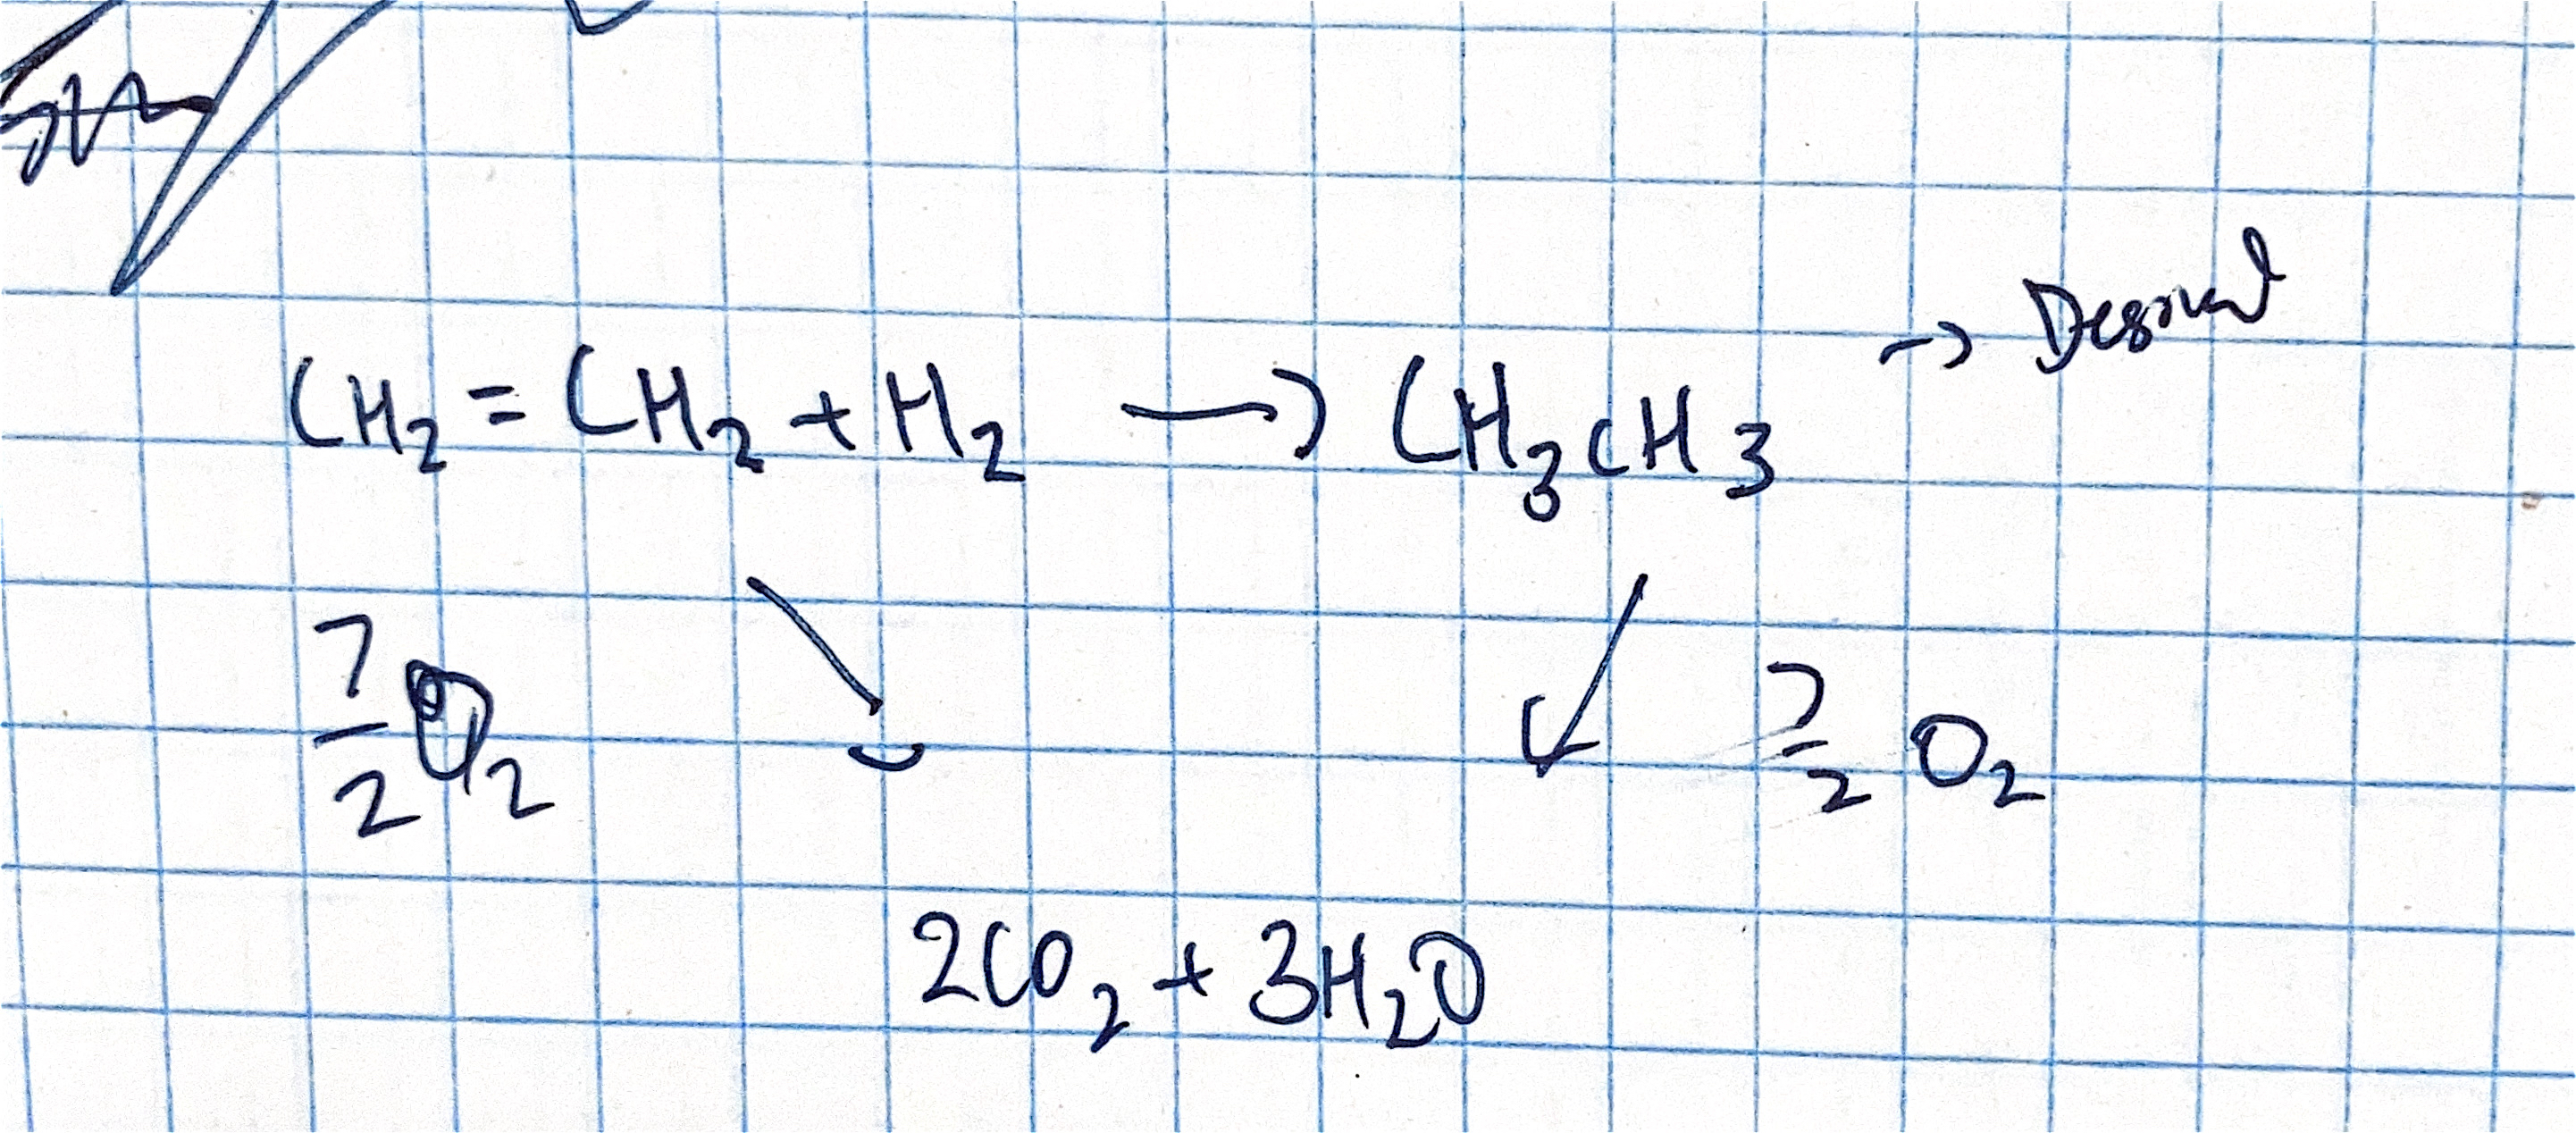
\includegraphics[width=\textwidth]{../images/1.2fig1.jpg}
	\caption{Given this image, find the equations to perform Hess's Law}
	\label{fig:image}
\end{figure}

Desired Equation:
$$CH_2=CH_2 + H_2 \rightarrow CH_3CH_3$$

Using the image above we can get the following reaction equations that allow us to use Hess's Law:

\begin{enumerate}
\item $CH_2=CH_2 + O_2 \rightarrow 2CO_2 + 2H_2O\ |\ \triangle{H} = -1411kJ/mol$
\item $CH_3CH_3 + \frac{7}{2}O_2 \rightarrow 2CO_2 + 3H_2O\ |\ triangle{H} = +1561kJ/mol$
\item $H_2 + \frac{1}{2}O_2 \rightarrow H_2O\ |\ \triangle{H} = -285.8kJ/mol$
\end{enumerate}

\subsection{\textbf{Goal: Solve the linear system}}

The goal is to cancel out a bunch of elements just as Hess's Law is solved! Wow, amazing...
The goal is to create a system of equations that cancels out when added. The \textbf{enthalpies} are summed up to find the \underline{desired} or \underline{final} enthalpy.\\

\textbf{Final Equation}

$CH_2=CH_2+H_2\rightarrow CH_3CH_3\ |\ \triangle{H}=-135.8kJ/mol$

\pagebreak

\section{$\star$ Enthalpy of Formation}

\textbf{Enthalpy of formation} is the energy required to form a compound; how much energy is added or revmoed to form it

\begin{itemize}
\item any element in standard from (includign diatomic gasses) have a $\triangle{H}_f = 0$
\end{itemize}

\subsection{Finding the Enthlapy of Formation}

Equation

$$C+H_2+O_2 \rightarrow C_3H_7OH$$

\begin{itemize}
\item left side $\triangle{H}_f = 0$ because all elements are in their standard state
\item find right side then
\end{itemize}

\centering
$\triangle{H}_f = -84kJ/mol(CH_3CH_3) - [52kJ/mol(C_2H_4) + 0(H_2)]$\\
$\triangle{H}_f = \triangle{H}_{f,pro} - \triangle{H}_{f,rea}$\\
$\triangle{H}_f = -126kJ/mol(C_3H_7OH)$

\end{document}














